%!TEX root = main.tex

% \begin{document}
\section{Operads}\label{sec:operads}
    % \cite{ha}
    Operads are a concept that originally occurred when studying loop spaces. 
    Let $\Omega X$ be the space of based loops in a topological space $X$. 
    Its structure reflects an interesting form of algebraic composition. 
    The composition of loops is only associative up to homotopy equivalence meaning 
    that loop spaces behave like a monoid in a homotopy-theoretic
    sense, but not in a strict algebraic sense. An operad can be thought of 
    as a structure that encodes a family of operations, each of which has a 
    certain number of inputs, and a way to compose these operations together. 
    The composition of operations in an operad satisfies associativity and unit laws. 

    Let $\alpha \colon [0,1] \to X$ and $\beta\colon [0,1] \to X$ be loops in $X$ having the same base point $x_0$. Their composition $\beta \circ \alpha$ is usually defined by splitting the unit interval in half, i.e.
    \[ \beta \circ \alpha (s) \coloneqq
        \begin{cases}
            \alpha(2s) & \text{for } s \in [0,\frac{1}{2}] \\
            \beta(2s-1) & \text{for } s \in (\frac{1}{2},1].
        \end{cases}
    \]

    This concatenation in itself is not associative; consider $\alpha, \beta, \gamma \in \Omega X$. Then by the given definition $\gamma \circ (\beta \circ \alpha)$ and $(\gamma \circ \beta) \circ \alpha$ are different maps:
     \[ \gamma \circ (\beta \circ \alpha) (s) =
        \begin{cases}
            \alpha(4s) & \text{for } s \in [0,\frac{1}{4}] \\
            \beta(4s-1) & \text{for } s \in (\frac{1}{4}, \frac{1}{2}] \\
            \gamma(2s-1) & \text{for } s \in (\frac{1}{2}, 1]      
        \end{cases}
    \]
    \[ (\gamma \circ \beta) \circ \alpha (s) =
        \begin{cases}
            \alpha(2s) & \text{for } s \in [0,\frac{1}{2}] \\
            \beta(4s-2) & \text{for } s \in (\frac{1}{2}, \frac{3}{4}] \\
            \gamma(4s-3) & \text{for } s \in (\frac{3}{4}, 1]
        \end{cases}
    \]
    The choice of splitting the unit intervall in half is merely a convention. Hence, composition of loops can be thought of as splitting intervals in an arbitrary manner; or in other words embedding unit intervals into a unit interval such that the image of the inner intervals are disjoint.

    \[
        \big[[I_1] \dots [\quad I_i \quad ] \dots [\: I_n \: ]\big]
    \]
    
    So, for an ordered family of loops $\{\alpha_i \colon I_i \to X\}_{1 \leq i \leq n}$ there is for each order preserving concatenation $\beta$ a unique map $f \in \Emb(I_1, \dots, I_n, I)$ such that $\beta \circ f (I_i) = \alpha_i$ for all $1 \leq i \leq n$. We denote the set of embeddings by $\E(n) = \Emb(I_1, \dots, I_n, I)$ for each $n \in \N$.
    For every $(f_k, (f_{j_i})_{1 \leq i \leq k}) \in  \E(k) \times \E(j_1) \times \dots \times \E(j_k)$ we obtain an embedding $f \in \E(j_1 + \dots + j_k)$ by defining $f = f_k \circ (f_{j_1} \sqcup \dots \sqcup f_{j_k})$. This defines a composition map 
    \[
        \gamma \colon \E(k) \times \E(j_1) \times \dots \times \E(j_k) \to \E(j_1 + \dots + j_k)
    \]
    Since the composition of maps is associative the following diagram commutes:
    \begin{center}
        \begin{tikzcd}
            \E(k) \otimes (\prod_{s=1}^k \E(j_s)) \times (\prod_{r=1}^j \E(i_r)) \arrow[rr, "\gamma \otimes \id"] \arrow[dd, "s"']               &  & \E(j) \times (\prod_{r=1}^j \E(i_r)) \arrow[d, "\gamma"]   \\                                                                           &  & \E(i)   \\
            \E(k) \otimes (\prod_{s=1}^k (\E(j_s) \times \prod_{q=1}^{j_s} \E(i_{g_{s-1}+q})) \arrow[rr, "\id \times \gamma^s"'] &  & \E(k) \times ((\prod_{s=1}^k \E(h_s)) \arrow[u, "\gamma"']
        \end{tikzcd}
    \end{center}
    where $s$ shuffles the cartesian product and
    \[
                n,  \ j_1, \dots, j_k, \ i_1, \dots, i_j \in \N
            \]
            with
            \[
                \sum_{1 \leq s \leq k} j_s = j, ~ \sum_{1 \leq r \leq j} i_r = i, \ g_s = \sum_{0 \leq l \leq s} j_l \ \text{and} \ h_s = \sum_{1 \leq q \leq j_s} i_{g_{s-1}+q}.
            \]
    
    Further composing with the identity embedding in $\E(1)$ does nothing. Thus, we have seen our 
    first example of an operad, providing a framework in which the composition of loop spaces 
    satisfies associativity.

    In this way, operads provide a more general and flexible formalism for capturing the algebraic 
    structures found in loop spaces and other topological constructs where composition occurs up to 
    homotopy. Similarly to monoids that can be considered as single object categories, operads can be 
    considered as single object multicategories. 
    In this section, we will introdue the notion of a planar and a symmetric operad as they were 
    introduced by May in \cite{may}. Then, we will move on to the more general notion of a colored 
    operad following \cite{ha}. We will establish a second equivalent definition of a colored operad 
    that is purely categorical, meaning we can therefore also phrase it in an $\infty$-categorial context.
    In the next section we will then consider braided operads and we work towards defining braided 
    colored operads. Ultimately, our goal is a purely functorial definition of a braided colored operad 
    such that we can lift the concept to an $\infty$-categorial context as well.

    \subsection{Planar and Symmetric Operads}

    From now on, unless it is stated otherwise, let $\C$ be a symmetric monoidal category with tensor product $\otimes$ and tensor unit $\I$. For an object $C$ in $\C$, we write $C^j$ for the $j$-th tensor power of $C$.

    \begin{defin}\label{planaroperad}
        A {\em planar operad} $\P$ in $\C$ consists of a family of objects $(\P(j))_{j \in \N}$ together with a unit morphism $\eta \colon k \rightarrow \P(1)$ and a product morphism
        \[
            \gamma \colon \P(k) \otimes \P(j_1) \otimes \cdots \otimes \P(j_k) \rightarrow \P(j),
        \]
        where $\sum_{1 \leq i \leq k} j_i = j$ such that the following associativity and unitality constraints hold:
        \begin{itemize}
            \item For any choice of integers
            \[
                n,  \ j_1, \dots, j_k, \ i_1, \dots, i_j
            \]
            with
            \[
                \sum_{1 \leq s \leq k} j_s = j, ~ \sum_{1 \leq r \leq j} i_r = i, \ g_s = \sum_{0 \leq l \leq s} j_l \ \text{and} \ h_s = \sum_{1 \leq q \leq j_s} i_{g_{s-1}+q}
            \]
            % \sum_{1 \leq s \leq k} j_s = j$, $\sum_{1 \leq r \leq j} i_r = i$, $g_s = \sum_{0 \leq l \leq s} j_l$ and $h_s = \sum_{1 \leq q \leq j_s} i_{g_{s-1}+q}$ 
            
            the following diagram commutes:
                \begin{center}
                \begin{tikzcd}
                    \P(k) \otimes (\bigotimes_{s=1}^k \P(j_s)) \otimes (\bigotimes_{r=1}^j \P(i_r)) \arrow[rr, "\gamma \otimes \id"] \arrow[dd, "s"']               &  & \P(j) \otimes (\bigotimes_{r=1}^j \P(i_r)) \arrow[d, "\gamma"]   \\                                                                           &  & \P(i)   \\
                    \P(k) \otimes (\bigotimes_{s=1}^k (\P(j_s) \otimes \bigotimes_{q=1}^{j_s} \P(i_{g_{s-1}+q})) \arrow[rr, "\id \otimes (\otimes_s \gamma)"'] &  & \P(k) \otimes ((\bigotimes_{s=1}^k \P(h_s)) \arrow[u, "\gamma"']
                \end{tikzcd}
                \end{center}
                where $s$ shuffles the entries of the tensor product.
        
                
            \item For all $j \in \N$ the following diagrams commute:
                \begin{center}
                \begin{tikzcd}
                    \P(j) \otimes k^j \arrow[r, "\cong"] \arrow[d, "\id \otimes (\otimes_j \eta)"'] & \P(j) &  & k \otimes \P(j) \arrow[d, "\eta \otimes \id"'] \arrow[r, "\cong"] & \P(j) \\
                    \P(j) \otimes \P(1)^j \arrow[ru, "\gamma"']                                     &      &  & \P(1) \otimes \P(j) \arrow[ru, "\gamma"']                         &     
                \end{tikzcd}
                \end{center}
        \end{itemize}
    \end{defin}

    \begin{egs}\label{egs_planar_operad}
        Let us consider some examples of planar operads in a symmetric monoidal category $\C$:
        \begin{enumerate} 
            \item Later we will define what it means to be an algebra over an operad. The \textit{associative operad} 
            $\Ass$ is the operad whose algebras are associative monoids. The associative planar operad in $\C$ is 
            the operad $\Ass_{\C}(n) = \I$ for all $i \in \N$ with $\id_{\I}$ being the unit and the composition 
            map being the canonical isomorphism. Hence, for $\C=\Set$, the category of sets equipped with 
            the cartesian symmetric monoidal structure, we obtain exactly one $n$-ary operation for each $n$: $\Ass_{\Set}$
            is defined by $\Ass_{\Set}(n) = \ast$ for all $n$. Similarly, for $\C = \Vect_K$ we get the free abelian 
            vector space over $\ast$, i.e. $K$.
            
        
            \item At the beginning of the section we already saw that the concatenation of loops defines an operad: 
            Let $\C = \Top$. Then we can define the \textit{operad of little interval} $\E$ as
            \[
                \E(n) = \Emb(I_1, \dots, I_n, I),
            \]
            the set of orientation-preserving embeddings of $n$ disjoint intervals into the unit interval $I$. 
            We equip $\E(n)$ with the subspace topology of $\R^n$. Composition is defined 
            by inserting the intervals into another interval as we have seen above.
            
            \item For $\C$ being closed, i.e. having an internal hom functor $\HHom(-, -)$, we can define 
            another planar operad $\End_X$ for any object $X \in \C$:
            \[
                \End_X(n) \coloneqq \HHom(X^{\otimes n}, X)
            \]
            The unit morphism $\eta$ is given by the image of $\id_X$ under the adjunction:
            \[
                \Hom(X,X) \cong \Hom(I, \HHom(X,X))
            \]
            Further, the composition morphism 
            \[
                \HHom(X^{\otimes k}, X) \otimes \bigotimes_s \HHom(X^{\otimes j_s}, X) \to \HHom(X^{\otimes j}, X)
            \]
            is given by composition:
            
            \begin{center}
                \begin{tikzcd}
                    {\HHom(X^{\otimes k}, X) \otimes \bigotimes_s \HHom(X^{\otimes j_s}, X)} \arrow[d] \\ {\HHom(X^{\otimes k}, X) \otimes \HHom(X^{\otimes j}, X^{\otimes k})} \arrow[d] \\
                    {\HHom(X^{\otimes j}, X)}
                \end{tikzcd}          
            \end{center}
        
            We call $\End_X$ the {\em endomorphism operad over} $X$.

        \end{enumerate}
    \end{egs}

    For another example of an operad, which we will encounter quite a lot in the following, we need to recall the definition of the braid group first.

    \begin{defin}
        For each integer $n > 2$ we define the {\em braid group} on $n$ strands as the group with $n-1$ generators $\sigma_1, \dots ,\sigma_{n-1}$ satisfying the following relations:
        \begin{align*}
            \sigma_i \sigma_j & = \sigma_j \sigma_i & \text{for } &|i-j|>1\\
            \sigma_i \sigma_{i+1} \sigma_i & = \sigma_{i+1} \sigma_i \sigma_{i+1} & \text{for } &1 \leq i \leq n-2
        \end{align*}
        For $n=2$ we define $B_2$ as the free group with one generator and let $B_0 = B_1 = \{1\}$ be the trivial group.
    \end{defin}

    \begin{rem}
        The name braid group $B_n$ makes sense when we consider the following depiction of the group for $0 \leq i, j \leq n$ with $i +1 < j$:

        \begin{center}
                \begin{tikzpicture}
                    \pic[
                    braid/number of strands=6,
                    braid/strand 2/.style={white},
                    braid/strand 5/.style={white},
                    name=coordinates,
                    ] at (0,0) {braid={s_3}};
                    \node[at=(coordinates-rev-2-e)] {$\dots$};
                    \node[at=(coordinates-rev-3-e), below=3pt] {$i$};
                    \node[at=(coordinates-rev-4-e), below=3pt] {$i+1$};
                    \node[at=(coordinates-rev-5-e)] {$\dots$};
                    \node[anchor=center] at (-0.5,-0.75) {$\sigma_i = \quad $};
            \end{tikzpicture}
            \medskip
                \begin{tikzpicture}
                    \pic[
                    braid/number of strands=9,
                    braid/strand 2/.style={white},
                    braid/strand 5/.style={white},
                    braid/strand 8/.style={white},
                    name=coordinates,
                    ] at (0,0) {braid={s_3-s_6}};
                    \node[at=(coordinates-rev-2-e)] {$\dots$};
                    \node[at=(coordinates-rev-3-e), below=3pt] {$i$};
                    \node[at=(coordinates-rev-4-e), below=3pt] {$i+1$};
                    \node[at=(coordinates-rev-5-e)] {$\dots$};
                    \node[at=(coordinates-rev-6-e), below=3pt] {$j$};
                    \node[at=(coordinates-rev-7-e), below=3pt] {$j+1$};
                    \node[at=(coordinates-rev-8-e)] {$\dots$};
                    \node[anchor=center] at (-1,-0.75) {$\sigma_i  \circ \sigma_j = \quad $};
                    \node[anchor=center] at (9,-0.75) {$\quad = \sigma_j \circ \sigma_i \quad $};
            \end{tikzpicture}
            \medskip
                    \begin{tikzpicture}
                    \pic[
                    braid/number of strands=7,
                    braid/strand 4/.style={white},
                    % % braid/strand 5/.style={white},
                    % braid/strand 6/.style={white},
                    name=coordinates,
                    ] at (0,0) {braid={s_1-s_6 s_2-s_5 s_1-s_6}};
                    % \node[at=(coordinates-rev-2-e)] {$\dots$};
                    \node[at=(coordinates-rev-1-e), below=3pt] {$i$};
                    \node[at=(coordinates-rev-2-e), below=3pt] {$i+1$};
                    \node[at=(coordinates-rev-3-e), below=3pt] {$i+2$};
                    \node[at=(coordinates-rev-5-e), below=3pt] {$i$};
                    \node[at=(coordinates-rev-6-e), below=3pt] {$i+1$};
                    \node[at=(coordinates-rev-7-e), below=3pt] {$i+2$};
                    % \node[at=(coordinates-rev-5-e)] {$\dots$};
                    % \node[at=(coordinates-rev-6-e), below=3pt] {$j$};
                    % \node[at=(coordinates-rev-7-e), below=3pt] {$j+1$};
                    % \node[at=(coordinates-rev-6-e)] {$\dots$};
                    \node[anchor=center] at (-1.5,-1.8) {$\sigma_i  \circ \sigma_{i+1} \circ \sigma_{i} = \quad $};
                    \node[anchor=center] at (7.75,-1.8) {$\quad = \sigma_{i+1} \circ \sigma_i \circ \sigma_{i+1} \quad $};
                    \node[anchor=center] at (3,-1.8) {$=$};
            \end{tikzpicture}
            \end{center}
    Further details on how this is defined formally can be found in \cite{hopf}. 
    \end{rem}

    We state some facts about braid groups that are known and can for example be found in \cite{yau}.
    
    \begin{rem}\label{braidfacts}
        \begin{enumerate}
            \item There is a projection, which we denote by $\pi \colon B_n \to S_n$, that adds the condition $\sigma_i^2 = \id$.
            \item The direct sum homomorphism 
            \[
                \bigoplus_S \colon S_{k_1} \times \dots \times S_{k_n} \to S_{k_1 + \dots + k_n}
            \]
            can be lifted to the braid groups:
            \[
                \bigoplus_B \colon B_{k_1} \times \dots \times B_{k_n} \to B_{k_1 + \dots + k_n}
            \]
            such that $ \bigoplus_B \circ \pi = (\pi)^k \circ \bigoplus_S$.
            Geometrically, $b_1 \oplus \dots \oplus b_n \in B_{k_1 + \dots k_n}$ describes the braid that places $b_1, \dots, b_n$ side by side from left to right.
            \item For $n \geq 1$ and $k_1, \dots, k_n \in \N$, the block permutation map
            \[
                (-)_S(k_1, \dots k_n) \colon S_n \to S_{k_1 + \dots + k+n}
            \] can be lifted to the braid groups:
            \[
                (-)_B(k_1, \dots k_n) \colon B_n \to B_{k_1 + \dots + k_n}
            \]
            such that $(-)_B(k_1, \dots k_n) \circ \pi = \pi \circ (-)_S(k_1, \dots k_n)$. Geometrically, for $b \in B_n$, the corresponding block braid $b(k_1, \dots, k_n)$ is obtained by replacing the $i$-th strand by $k_i$ many parallel strands for $1 \leq i \leq n$.
            \item Let $\sigma, \rho \in B_n$ and $\tau_j \in B_{k_j}$ for $1 \leq j \leq n$. Then the following hold in $B_{k_1 + \dots + k_n}$:
            \begin{align*}
                (\sigma \rho)(k_1, \dots, k_n) &= \sigma(k_{\bar{\rho}^{-1}(1)}, \dots, k_{\bar{\rho}^{-1}(n)}) \cdot \rho(k_1, \dots, k_n) \\
                \sigma(k_1, \dots, k_n) \cdot (\tau_1 \oplus \dots \oplus \tau_n) &= (\tau_{\bar{\sigma}^{-1}(1)} \oplus \dots \oplus \tau_{\bar{\sigma}^{-1}(n)} \cdot \sigma(k_1, \dots, k_n)
            \end{align*}
            where $\bar{\sigma} + \pi(\sigma)$ and $\bar{\rho} + \pi(\rho)$.
        \end{enumerate}
    \end{rem}
    
    \begin{eg}\label{braidop}
        Let $\B$ be the {\em braid operad} defined by:
        \[
            \B(n) \coloneqq B_n,
        \]
        where $B_n$ denotes the braid group on $n$ strands. The composition morphism 
        \begin{align*}
            \gamma \colon B_k \times B_{j_1} \times \dots \times B_{j_k} &\to B_{j} \\
            (\tau, (\sigma_i)_{1 \leq i \leq k}) &\mapsto \tau(\sigma_1 \oplus \dots \oplus \sigma_k)
        \end{align*}
        where $\tau(\sigma_1 \oplus \dots \oplus \sigma_k)$ denotes the braid that $\tau$-braids $k$ many block braids $\sigma_1, \dots, \sigma_k$ as if they where strands in $B_k$.
        
        So for the compositon map 
        \[
            B_2\times B_2 \times B_2 \to B_4
        \]
        let us observe what happens with the following element in $B_2\times B_2 \times B_2$:
        \begin{center}
        \begin{tikzpicture}[
            braid/.cd,
            strand 1/.style={black},
            strand 2/.style={black},
            strand 3/.style={blue},
            strand 4/.style={magenta},
            strand 5/.style={red},
            strand 6/.style={green},
            ]
            \pic at (0,0) {braid={s_1-s_3-s_5}};
        \end{tikzpicture}
        \end{center}
        After applying the composition map we obtain the following braiding:
        \begin{center}
        \begin{tikzpicture}[
            braid/.cd,
            strand 1/.style={blue},
            strand 2/.style={magenta},
            strand 3/.style={red},
            strand 4/.style={green},
            ]
            
            \pic at (0,0) {braid={s_1-s_3 s_{1,2,3} s_{2,3,4}}};
        \end{tikzpicture}
        \end{center}
        The associativity and unitality conditions follow from the group conditions.
    \end{eg}

    \begin{defin}
        Let $\P, \P'$ be planar operads in a symmetric monoidal category $\C$. A {\em morphism of planar operads} $\beta \colon \P \to \P'$ consists of morphisms $\beta_n \colon P(n) \to \P'(n)$ for all $n \in \N$ such that the following diagrams commute:
        \begin{center}
            \begin{tikzcd}
                \P(k) \otimes \P(j_1) \otimes \dots \otimes \P(j_k) \arrow[rr, "\beta_k \otimes \beta_{j_1} \otimes \dots \otimes \beta_{j_k}"] \arrow[d, "\gamma"'] &  & \P'(k) \otimes \P'(j_1) \otimes \dots \otimes \P'(j_k) \arrow[d, "\gamma'"] \\
                \P(j) \arrow[rr, "\beta_j"]                                                                                                                         &  & \P'(j)                                                                     
            \end{tikzcd}
        \end{center}
        \begin{center}
            \begin{tikzcd}
                                         & k \arrow[ld, "\eta"'] \arrow[rd, "\eta'"] &        \\
            \P(1) \arrow[rr, "\beta_1"] &                                           & \P'(1)
            \end{tikzcd}
        \end{center}
    \end{defin}
    Therefore, for any closed symmetric monoidal category $\C$ the planar operads and their morphisms form a category $\Plop_{\C}$.

    \medskip

    When we later discuss operads, we will seldom focus on planar operads but will work with symmetric operads instead.

    \begin{defin}\label{operad}
        A {\em (symmetric) operad} $\O$ in $\C$ is a planar operad as defined in \ref{planaroperad} with an action of $S_n$ on $\O(n)$ together with the following equivariance condition: 
           Let $\sigma(j_1, \cdots, j_k) \in S_j$ denote the element that permutes $k$ blocks of length $j_l$ for $1 \leq l \leq k$. Then, the following diagram commutes:
                \begin{center}
                \begin{tikzcd}
                    \O(k) \otimes \O(j_1) \otimes \cdots \otimes \O(j_k) \arrow[d, "\gamma"'] \arrow[rr, "\sigma \otimes \sigma^{-1}"] &  & \O(k) \otimes \O(j_{\sigma(1)}) \otimes \cdots \otimes \O(j_{\sigma(k)}) \arrow[d, "\gamma"] \\
                    \O(j) \arrow[rr, "\sigma(j_1 \cdots j_k)"']                                                                                        &  & O(j).                                                                    
                \end{tikzcd}
                \end{center}      

            Furthermore, let $\tau_l \in S_{j_l}$ and $\tau_1 \oplus \cdots \oplus \tau_k$ denotes the sum of permutations on $k$ blocks of length $j_l$ for $1 \leq l \leq k$. Then the following diagram commutes:
                
                \begin{center}
                \begin{tikzcd}
                    \O(k) \otimes \O(j_1) \otimes \cdots \otimes \O(j_k) \arrow[d, "\gamma"'] \arrow[rr, "\id \otimes \tau_1 \otimes \cdots \otimes \tau_k"] &  & \O(k) \otimes \O(j_1) \otimes \cdots \otimes \O(j_k) \arrow[d, "\gamma"] \\
                    \O(j) \arrow[rr, "\tau_1 \oplus \cdots \oplus \tau_k"']                                                                                &  & \O(j).                                                                                     
                \end{tikzcd}
                \end{center}
    \end{defin}

    As already mentioned we introduce operads as a tool to generally encode algebraic structure.
        
    \begin{defin}
        Let $\O$ be an operad in $C$. An $\O${\em -algebra} is an object A in $C$ with maps
        \[
            \theta \colon \O(j) \otimes A^j \rightarrow A
        \]
        for $j \in \N$ such that the following associativity, unitality and equivariant conditions hold:
        \begin{itemize}
            \item Associative:
                \begin{center}
                    \begin{tikzcd}
                        \O(k) \otimes \O(j_1) \otimes \cdots \otimes \O(j_k) \otimes A^j \arrow[rr, "\gamma \otimes \id"] \arrow[dd, "s"'] &  & \O(j) \otimes A^j \arrow[d, "\theta"]  \\
                        &  & A  \\
                        \O(k) \otimes (\bigotimes (\O(j_l) \otimes A^{j_l})) \arrow[rr, "\id \otimes \theta^k"']               &  & \O(k) \otimes A^k \arrow[u, "\theta"']
                    \end{tikzcd}
                \end{center}
            \item Unital:
                \begin{center}
                    \begin{tikzcd}
                        \I \otimes A \arrow[d, "\eta \otimes \id"'] \arrow[r, "\cong"] & A \\
                        \O(1) \otimes A \arrow[ru, "\theta"']                          &  
                    \end{tikzcd}
                \end{center}
            \item Equivariant:
                For all $j \in \N$ and $\sigma \in S_j$:
                \begin{center}
                    \begin{tikzcd}
                        \O(j) \otimes A^j \arrow[rr, "\sigma \otimes \sigma^{-1}"] \arrow[rd, "\theta"'] &   & \O(j) \otimes A^j \arrow[ld, "\theta"] \\
                        & A &     
                    \end{tikzcd}
                \end{center} 
        \end{itemize}
    \end{defin}

    \begin{defin}\label{module}
        Let $\O$ be an operad in $\C$, $A$ an $\O$-algebra. We call an object $M$ in $\C$ with maps
        \[
            \omega \colon \O(j) \otimes A^{j-1} \otimes M \rightarrow M 
        \]
        an $A${\em-module} if it satisfies the following associativity, unitality and equivariance conditions:
        \begin{itemize}
            \item Associative: For all $\sum j_l = j$ in $\N$ the following diagrams commute:
                \begin{center}
                \begin{tikzcd}
                    \O(k) \otimes \O(j_1) \otimes \cdots \otimes \O(j_k) \otimes A^{j-1} \otimes M \arrow[rr, "\gamma \otimes \id"] \arrow[dd, "s"']                                   &  & \O(j) \otimes A^{j-1} \otimes M \arrow[d, "\omega"]  \\
                    &  & M  \\
                    \O(k) \otimes \left(\bigotimes_{l=1}^{k-1} \O(j_l) \otimes A^{j_l}\right) \otimes \O(j_k) \otimes A^{j_k -1} \otimes M \arrow[rr, "\id \otimes \theta^{k-1} \otimes \omega"'] &  & \O(k) \otimes A^{k-1} \otimes M \arrow[u, "\omega"']
                \end{tikzcd}
                \end{center}
                
            \item Unital:
                \begin{center}
                \begin{tikzcd}
                    \I \otimes M \arrow[r, "\cong"] \arrow[d, "\eta \otimes \id"'] & M \\
                    \O(1) \otimes A^0 \otimes M \arrow[ru, "\omega"']              &  
                \end{tikzcd}
                \end{center}
        
            \item Equivariant: For all $j \in \N$ and $\sigma \in S_{j-1} \subset S_j$, the following diagram commutes:
                \begin{center}
                \begin{tikzcd}
                    \O(j) \otimes A^{j-1} \otimes M \arrow[rd, "\omega"'] \arrow[rr, "\sigma \otimes \sigma^{-1} \otimes \id"] &   & \O(j) \otimes A^{j-1} \otimes M \arrow[ld, "\omega"] \\
                     & M &                                                    
                \end{tikzcd}
                \end{center}
        \end{itemize}
    \end{defin}

    \begin{rem}
        We can of course also define algebras over planar operads by dropping the equivariance condition as there is no symmetric group action. So, algebras over the operad $\Ass$ which we defined in \ref{egs_planar_operad} are indeed monoids since the corresponding squares commute due to canonical isomorphisms:
            \begin{center}
                \begin{tikzcd}
                    \Ass(2) \otimes \Ass(2) \otimes \Ass(1) \otimes A^3 \arrow[rr, "\cong"] \arrow[dd, "\cong"'] &  & \Ass(3) \otimes A^3 \arrow[d, "\theta"]  \\
                    &  & A  \\
                    \Ass(2) \otimes (\Ass(2) \otimes A^2) \otimes (\Ass(1) \otimes A)) \arrow[rr, "\id \otimes \theta^2"']               &  & \Ass(2) \otimes A^2 \arrow[u, "\theta"']
                \end{tikzcd}
            \end{center}  

            \begin{center}
                \begin{tikzcd}
                    \Ass(2) \otimes \Ass(1) \otimes \Ass(2) \otimes A^3 \arrow[rr, "\cong"] \arrow[dd, "\cong"'] &  & \Ass(3) \otimes A^3 \arrow[d, "\theta"]  \\
                    &  & A  \\
                    \Ass(2) \otimes (\Ass(1) \otimes A) \otimes (\Ass(2) \otimes A^2)) \arrow[rr, "\id \otimes \theta^2"']               &  & \Ass(2) \otimes A^2 \arrow[u, "\theta"']
                \end{tikzcd}
            \end{center}  
    \end{rem}
    
    \begin{egs}
        \begin{enumerate} \label{egop}
            \item A natural question is whether the associative planar operad and the associative operad in a category $\C$ coincide.
            % However, this is not the case. 
            For $\C = \Set$, we can equip the associative operad
            $$\Ass_{\Set}^{\text{planar}}(n) = \ast$$ 
            with the trivial action of $S_n$. Yet this appears to be too restrictive:
            The equivariance condition implies that algebras over this operad are not just monoids but commutative monoids. To distinguish operations after acting by $S_n$, we can think of a more suited candidate: $\Ass(n)=S_n$ for all $n \in \N$ where $S_n$ acts on $\Ass(n)$ by translation. The composition map is defined by considering a sum of permutations and then permuting $k$ blocks of length $j_i$ for $1 \leq i \leq k$: 
            \begin{align*}
                \gamma \colon \Ass(k) \times \Ass(j_1) 
                \times \dots \times \Ass(j_k) & \to \Ass(k)\\
                (\sigma, \tau_1, \dots, \tau_k) & \mapsto \sigma(\tau_1 \oplus \dots \oplus \tau_k) \\
            \end{align*}
            We might also refer to this operad as the symmetry operad $\S$ later on.
            
            \item The operad $\Comm_{\Set}(n) = \ast$ with the trivial action of $S_n$ is an interesting operad nevertheless as it is the {\em commutative operad} in the category $\Set$. The commutative operad in a category $\C$ is the operad such that its algebras are commutative monoids in $\C$. 
            
            \item The {\em little $n$-disk operad} $\dd_n$ is an important example of an operad in the category of topological spaces $\Top$.
            For all $n \in \N$ we will define $\dd_n(k)$ as a topological space representing the space of $k$ disjoint little disks inside the unit disk in the plane.
            Let $n \in \N$ and 
            \[
                \dd^n = \left\{ (r_1, \dots, r_n) \in \R^n \colon r_1^2 + \dots + r_n^2 \leq 1\right\} \subset \R^n
            \]
            is the closed unit $n$-disk. A little $n$-disk is defined as the embedding $f \colon \dd^n \to \dd^n$ of the following form:
            \[
             f(r_1, \dots, r_n) \coloneqq (c_1, \dots, c_n) 
            + \lambda(r_1, \dots, r_n)
            \]
            for $(c_1, \dots, c_n) \in \dd^n$ and $\lambda \in \R$ such that
            \[
                0 < \lambda \leq 1 - \sum_{i=1}^{n} c_i^2.     
            \]
            We denote the interior of a little disk by $\inter(f)$ and define for $k > 0$:
            \[
                \dd_n(k) \coloneqq \left\{ f_1 \sqcup \dots \sqcup f_n \in C\left(\bigsqcup_{i=1}^k \dd^n, \dd^n\right) \colon \inter(f_i) \cap \inter(f_j) = \emptyset \text{ for all } i \not= j\right\} 
            \]
            We equip $C\left(\bigsqcup_{i=1}^k \dd^n, \dd^n\right)$ with the compact-open topology and $\dd_n(k)$ with the subspace topology. $\dd_n(0)$ is the one point space.
            % Each little disk is determined by the position of its center and its radius. Therefore, the space $\dd_n(n)$ is an open subset of $\R^{3n}$.
            % , because:
            % \begin{itemize}
            %     \item The center of each disk is described by two coordinates in $ \R^2$ (representing the plane), and
            %     \item Each disk’s radius is a positive real number in $\R$.
            % \end{itemize}
            % Thus, $\dd_n(n)$ is a manifold of dimension $3n$.
            There is an operad structure to be defined on
            \[
                \dd_n = \left\{\dd_n(k)\right\}_{k \geq 0}.
            \]
                        
            The construction of the composition map
            \[
            \gamma: \dd_n(k) \times \dd_n(l_1) \times \cdots \times \dd_n(l_k) \to \dd_n(l_1 + \cdots + l_k)
            \]
            is geometrically interpreted as:
            \begin{itemize}
                \item Start with a configuration in $\dd_n(k)$, which gives $k$ disks inside the unit disk.
                \item Each of the $k$ disks is treated as a new "unit disk" in which a configuration from $\dd_n(l_1), \dd_n(l_2), \dots, \dd_n(l_k)$ can be inserted.
                \item The configurations from $\dd_n(l_1), \dd_n(l_2), \dots, \dd_n(l_k)$ are scaled down to fit inside the respective disks from the configuration in $\dd_n(k)$, and they are inserted.
                \item After placing all configurations inside the $k$ disks, the boundary are erased, yielding a new configuration in $\dd_n(n_1 + \dots + n_k)$.
            \end{itemize}
            
            \begin{center}
                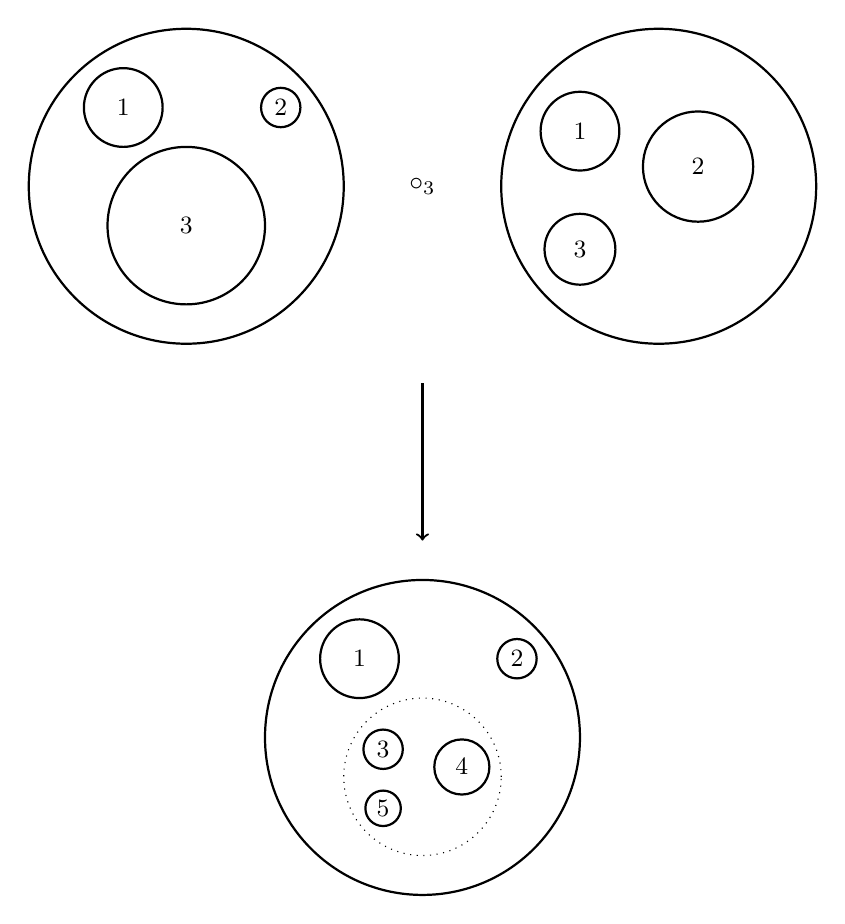
\begin{tikzpicture}
                    % First element (left)
                    \draw[thick] (-3,0) circle (2);
                    \draw[thick] (-3.8, 1) circle (0.5);
                    \draw[thick] (-1.8, 1) circle (0.25);
                    \draw[thick] (-3, -0.5) circle (1);
                    \node at (-3.8, 1) {\small $1$};
                    \node at (-1.8, 1) {\small $2$};
                    \node at (-3, -0.5) {\small $3$};
                
                    \node at (0,0) {$\circ_3$};
                
                    % Second element (right)
                    \draw[thick] (3,0) circle (2);
                    \draw[thick] (2,0.7) circle (0.5);
                    \draw[thick] (3.5,0.25) circle (0.7);
                    \draw[thick] (2,-0.8) circle (0.45);
                    \node at (2,0.7) {\small $1$};
                    \node at (3.5,0.25) {\small $2$};
                    \node at (2,-0.8) {\small $3$};
                
                
                    % Arrow between first two
                    \draw[->, thick] (0,-2.5) -- (0,-4.5); %node[midway, above] {\small Insert into $3$};
                
                    % Third element (bottom)
                    \draw[thick] (0,-7) circle (2);
                
                    \draw[thick] (-0.8, -6) circle (0.5);
                    \draw[thick] (1.2, -6) circle (0.25);
                    \draw[dotted] (0, -7.5) circle (1);
                
                    \draw[thick] (-0.5, -7.15) circle (0.25); 
                    \draw[thick] (0.5, -7.375) circle (0.35); 
                    \draw[thick] (-0.5, -7.9) circle (0.225);  
                    
                    \node at (-0.8, -6) {\small $1$};
                    \node at (1.2, -6) {\small $2$};
                    \node at (-0.5, -7.15) {\small $3$};
                    \node at (0.5, -7.375) {\small $4$};
                    \node at (-0.5, -7.9)  {\small $5$};
                \end{tikzpicture}
            \end{center}
            
            Formally, this means that for $(f, (g_i)_{1 \leq i \leq k}) \in \dd_n(l_1) \times \dd_n(l_2) \times \dots \times \dd_n(l_k)$ we define $\gamma((f, (g_i)_{1 \leq i \leq k}))$ via the following commuting diagram:

            \begin{center}
                \begin{tikzcd}
                    \bigsqcup_{j = 1}^l \dd^n \arrow[r, "{\gamma(f,(g_i)_{1 \leq i \leq k})}"] \arrow[d, "\cong"]                                                               & \dd^n                                 \\
                    \bigsqcup_{i =1}^k \left(\bigsqcup_{p =1}^{l_k} \dd^n \right) \arrow[r, "\bigsqcup g_i                                                             ~"] & \bigsqcup_{i =1}^k \dd^n \arrow[u, "f"]
                \end{tikzcd}
            \end{center}

            The unit is the identity configuration, where the single disk remains unchanged, i.e. the identity map $\id_{\dd^n} \in C\left(\dd^n, \dd^n\right)$.
            This satisfies the unitality condition for operads by definition, where inserting a single disk into another disk does not alter any configuration:
                $\gamma((f, (\id)_{1 \leq i \leq k})) = f$
            and 
                $\gamma((\id, g)) = g$.
            
            The composition map satisfies the associativity condition by definition.

            The disks are labeled, and there is an action of the symmetric group $S_k$ on $\dd_n(k)$, which permutes the labels of the disks: 
            For $f_1 \sqcup \dots \sqcup f_k \in \dd_n(k)$ and $\sigma \in S_k$:
            \[
                \sigma (f_1 \sqcup \dots \sqcup f_k) \coloneqq f_{\sigma(1)} \sqcup \dots \sqcup f_{\sigma(k)}
            \]

            The composition map $\gamma$ respects the action of $S_k$:
            For any $\sigma \in S_k$, $\tau_i \in S_{l_i}$ and $(f, (g_i)_{1 \leq i \leq k}) \in \dd_n(k) \times \dd_n(l_1) \times \cdots \times \dd_n(l_k)$
            we have by definition
            \begin{align*}
                \sigma \circ \gamma ((f, (g_i)_{1 \leq i \leq k})) &= \sigma\left(\bigsqcup_{i=1}^k f_i \circ g_i \right) \\
                &= \bigsqcup_{i=1}^k f_{\sigma(i)}\circ g_{\sigma(i)} \\
                &= \gamma \left( (f_{\sigma(1)} \sqcup \dots \sqcup f_{\sigma(k)}, g_{\sigma(1)}, \dots, g_{\sigma(k)}\right) \\
                &= \gamma \circ (\sigma \times \sigma^{-1}) ((f, (g_i)_{1 \leq i \leq k})) \\
            \end{align*}
            and 
            \begin{align*}
                (\tau_1 \oplus \dots \oplus \tau_k) \circ \gamma ((f, (g_i)_{1 \leq i \leq k})) &= (\tau_1 \oplus \dots \oplus \tau_k) \left(\bigsqcup_{i=1}^k f_i \circ g_i \right) \\
                &= \bigsqcup_{i=1}^k f_i \circ {\tau_i(g_i)} \\
                &= \gamma \left( (f, \tau_1(g_1), \dots, \tau_k(g_k)\right) \\
                &= \gamma \circ (\tau_1 \times \dots \times \tau_k) ((f, (g_i)_{1 \leq i \leq k})). \\
            \end{align*}
        
            
            % Hence, the following diagrams commutes:
            % \[
            %     \begin{tikzcd}
            %         \dd_n(k) \times \dd_n(l_1) \times \cdots \times \dd_n(l_k) \arrow[r, "\sigma \times \sigma^{-1}"] \arrow[d, "\gamma"] & \dd_n(k) \times \dd_n(l_{\sigma(1)}) \times \cdots \times \dd_n(l_{\sigma(k)}) \arrow[d, "\gamma"] \\
            %         \dd_n(l) \arrow[r, "\sigma"] & \dd_n(l)
            %     \end{tikzcd}
            % \]
            % \begin{center}
            %     \begin{tikzcd}
            %         \dd_n(k) \times \dd_n(l_1) \times \cdots \times \dd_n(l_k) \arrow[d, "\gamma"'] \arrow[rr, "\id \times \tau_1 \times \cdots \times \tau_k"] &  & \dd_n(k) \times \dd_n(l_{\sigma(1)}) \times \cdots \times \dd_n(l_{\sigma(k)}) \arrow[d, "\gamma"] \\
            %         \dd_n(l) \arrow[rr, "\tau_1 \oplus \cdots \oplus \tau_k"']                                                                                &  & \dd_n(l)                                                                                  
            %     \end{tikzcd}
            % \end{center}


     
            
            % \item The Associahedra Operad
            % \item lie operad
        \end{enumerate}
    \end{egs}

%%%%%%%%%%%%%%%%%%%%%%%%%%%%%%%%%%%%%%%%%%%%%%%%%%%%%%%%%%%%%%%%%%%%%%%%%%%%%%%%%%%%%

    \subsection{Colored Operads}
    
    Following \cite{ha}, the goal of this section is to introduce colored operads in such a way that we 
    can define colored $\infty$-operads later on. A symmetric monoidal category is an 
    example of a colored operad. Thus, we will focus on this special case first. We will show that a symmetric 
    monoidal category can be defined in a purely functorial way. After that we will then follow this approach 
    and define the notion of a colored operad in a similar way.
    
    Let us start by introducing some terminology.
    
    \begin{defin}
        Let $P \colon \C \to \D $ be a functor of arbitrary categories and $f \colon x \to y$ a morphism in $\C$. We call $f$ {\em cartesian} if for any morphism $g \colon  z \to y$ in $\C$ and $\omega \colon P(z) \to P(x)$ in $\D$ with $P(f) \circ \omega = P(g)$, there exists a unique morphism $\omega' \colon z \to x$ in $\C$ such that $g = f \circ \omega'$ and $P(\omega')= \omega$. In diagrams we have:
        \begin{center}
            \begin{tikzcd}
            z \arrow[r, "g"] \arrow[d, "\exists!"', dotted] & y & {} \arrow[r, "P", shift right=9] & {} & P(z) \arrow[r] \arrow[d] & P(y) \\
            x \arrow[ru, "f"']                              &   &                                  &    & P(x) \arrow[ru]          &     
            \end{tikzcd}
        \end{center}
        And vice versa, we call $f$ {\em cocartesian} if we can flip arrows of the above case, i.e. for any morphism $g \colon  y \to z$ in $\C$ and $\omega \colon P(x) \to P(z)$ in $\D$ with $\omega \circ P(f) = P(g)$, there is a unique morphism $\omega' \colon x \to z$ such that $P(\omega')=\omega$ and $\omega' \circ f = g$. In a diagram this means the following:
        \[
            \begin{tikzcd}
                y \arrow[r] \arrow[rd, "f"'] & z                                & {} \arrow[r, "P"] & {} & P(y) \arrow[r] \arrow[rd] & P(z)           \\
                                             & x \arrow[u, "\exists!"', dotted] &                   &    &                           & P(x) \arrow[u]
            \end{tikzcd}
        \]
    \end{defin}

    Note that equivalently we can define a cocartesian morphism by requiring a bijection:
    \[
    \Hom_{\C}(y,z) \times_{\Hom_{\D}(P(y), P(z))} \Hom_{\D}(P(x), P(z)) \cong \Hom_{\C}(x,z)
    \]
    where $\Hom_{\C}(y,z) \times_{\Hom_{\D}(P(y), P(z))} \Hom_{\D}(P(x), P(z))$ is the pullback of applying the functor $P$ to $\Hom_{\C}(y,z)$ and precomposing with $P(f) \colon P(y) \to P(x)$.
    So, for the bijection we send a pair $(g, \omega)$ to the unique morphism $\omega'$ and vice versa we send a morphism $h \colon x \to z$ to the pair $(h \circ f, P(h))$.

    \begin{defin}
        Let $P \colon \C \to \D$ be a functor. $P$ is called a {\em (Grothendieck) fibration} if for every object y in $\C$ and morphisms $f' \colon x' \to P(y)$ there exists a cartesian morphism $f \colon x \to y$ such that $f' = P(f)$.
        We call $f$ a cartesian lift of $f'$ and $f'$ a cleavage.
        Dually we define the notion of a {\em (Grothendieck) cofibration}, i.e. $P$ is a cofibration if for every object $x$ in $\C$ and morphism $f' \colon P(x) \to y'$ there exists a cocartesian morphism $f \colon x \to y$ such that $P(f)=f'$.
    \end{defin}


    \begin{defin}\label{Cxdef}
        Let $\C$ be a symmetric monoidal category. We define a new category $\Cotimes$ in the following way:
        \begin{itemize}
            \item Objects of $\Cotimes$ are finite sequences $[C_1, \dots, C_n]$ where $C_i$ is an object in $\C$ for all $i$. It is possible that the sequence is empty.
            
            \item A morphismn $f \colon [C_1, \dots, C_n] \to [C_1', \dots, C_m']$ in $\Cotimes$ consists of a subset $S_f \subset \{1, \dots, n\}$, a map of finite sets $\alpha_f \colon S_f \to \{1, \dots, m\}$ and a family of morphisms
            
            $$\left\{f_j \colon \bigotimes_{\alpha_f(i)=j} C_i \to C_j'\right\}_{1 \leq j \leq m}$$
            
            in $\C$.
            
            \item Composition is defined as follows: Let 
            $$f \colon [C_1, \dots, C_n] \to [C_1', \dots, C_m'] \quad \text{and} \quad g \colon [C_1', \dots, C_m'] \to [C_1'', \dots, C_k'']$$ be morphisms in $\Cotimes$, then 
            
            $$g \circ f \colon [C_1, \dots, C_n] \to [C_1'', \dots, C_k'']$$
            
            is defined via $S_{g \circ f} = \alpha_f^{-1}(S_g)$,  $\alpha_{g \circ f} = \alpha_g \circ \alpha_f|_{S_{g \circ f}}$ and for all $1 \leq l \leq k$ we have:
            \[
                \bigotimes_{\alpha_{g \circ f}(i)= l} C_i \cong \bigotimes_{\alpha_g(j)=k} \bigotimes_{\alpha_g(i)=j} C_i \to \bigotimes_{\alpha_g(j)=k} C_j' \to C_l''.
            \]
        \end{itemize}
    \end{defin}

    Let $I$ be a finite set. We write $I_* = I \coprod {*}$.

    \begin{defin}
        We define $\Fin$, the {\em category of finite pointed sets}, as follows:
        \begin{itemize}
            \item For each $n \in \N$ we write $\langle n \rangle^{\circ} := \{1, \dots, n\}$. We define the objects of $\Fin$ as $ \langle n \rangle := \langle n \rangle^{\circ}_*$.
            \item A morphism $\alpha \colon \langle n \rangle \to \langle m \rangle$ is a map of finite sets where $\alpha(*)=*$
        \end{itemize}
    \end{defin}
    
      It is clear that this defines a category. Further note that this category is equivalent to the category of finite sets with a distinguished point since for any finite set $I$ we have an isomorphism $I_* \cong \langle n \rangle$, where $n$ is the cardinality of $I$. For all pairs of $1 \leq i \leq n$ we write $\rho^i \colon \langle n \rangle \to  \langle 1 \rangle$ for the morphism in $\Fin$ which is defined by
      \[
        \rho^i (j) = 
        \begin{cases}
            1 & i=j \\
            * & \text{else}.
        \end{cases}
      \]

      For any symmetric monoidal category $\C$ there exists a forgetful functor
      
      \[
      P \colon \Cotimes \to \Fin
      \]
      
      which sends a sequence $[C_1, \dots, C_n]$ to $\langle n \rangle$ and a morphism $f \colon [C_1, \dots, C_n] \to [C_1', \dots, C_m']$ to $\alpha \colon \langle n \rangle \to \langle m \rangle$ with
      \[\alpha (x) = \begin{cases}
          \alpha_f(x) & x \in S_f \\
          * & \text{else}.
      \end{cases}\]

    \begin{rem}
          Let $\C_0$ denote the trivial category of one object and one morphism. We claim that the forgetful functor $P \colon \C_0^{\otimes} \to \Fin$ is an isomorphism of categories. This holds, since for all morphisms in $\C_0^{\otimes}$ the family of morphisms $f_j$ in $\C_0$ are trivial, in other words there is nothing to forget. Hence, $\Fin$ is obtained as the simplest example of the construction of a $\Cotimes$ category.

          Furthermore, we note that the forgetful functor $P \colon \Cotimes \to \Fin$ can be obtained from a unique symmetric monoidal functor $F \colon \C \to \C_0$ using the functoriality of $F$.
    \end{rem}

    \begin{rem}
         For every object $\langle n \rangle$ we denote the fiber category by $\C_{\langle n \rangle}$, which is defined to be the pullback of the following diagram
        \begin{center}
            \begin{tikzcd}
                \Cotimes_{\langle n \rangle} \arrow[r, dashed] \arrow[d, dashed] & \Cotimes \arrow[d, "P"] \\
                \{\langle n \rangle\} \arrow[r, hook]                            & \Fin                   
            \end{tikzcd}
        \end{center}
        where $\{\langle n \rangle\}$ is interpreted as the trivial one object category. 
        In other words, $\C_{\langle n \rangle}$ consists of all collections of objects of length $n$ and all morphisms $f$ such that $\alpha_f = \id_{\langle n \rangle}$.    
    \end{rem}

    We are now ready to state two very important properties of the functor $P \colon \Cotimes \to \Fin$, which as it turns out is all we need to know.
    
    \begin{prop}\label{m1m2}
        \begin{enumerate}[(M1)]
            \item The forgetful functor $P \colon \Cotimes \to \Fin$ is a cofibration.
            \item We have that $\C \cong \Cotimes_{\langle 1 \rangle}$ and more precisely we obtain that $\Cotimes_{\langle n \rangle} \cong \C^n$ where $\C^n$ denotes the $n$-fold product of  copies of $\C$.
        \end{enumerate}
    \end{prop}

    \begin{proof}
        \begin{enumerate}[(M1)]
            \item Let $[C_1, \dots, C_n]$ be an object in $\Cotimes$ and $f' \colon \langle n \rangle \to \langle m \rangle$ a morphism in $\Fin$. We need to construct a cocartesian morphism $f \colon [C_1, \dots, C_n] \to [C_1', \dots, C_m']$ such that $P(f) = f'$.
            We define $\alpha_f \colon S_f\to \langle m \rangle^{\circ}$ as $\alpha_f := f'|_{S_f}$ where $S_f := f'^{-1}(\langle m \rangle^{\circ})$. Further we define a selection of objects in $\C$ for $1 \leq j \leq m$:
            \[
                C_j' := \begin{cases}
                    \bigotimes_{\alpha_f(i)=j} C_i & j \in \alpha_f(S_f)\\
                    \I & \text{else}
                \end{cases}
            \]
            For $f_j := \id_{C_j'}$ we have then constructed a well defined morphism 
            
            $$f \colon [C_1, \dots, C_n] \to [C_1', \dots, C_m']$$
            
            such that $P(f) = f'$. We are left to show that $f$ is indeed cocartesian.
            Therefore, let $g \colon [C_1, \dots, C_n] \to [C_1'', \dots, C_l'']$ be a morphism in $\Cotimes$ and $\omega' \colon \langle m \rangle \to \langle l \rangle$ a morphism in $\Fin$ such that $P(g) = \omega' \circ P(f)$. We need to find a unique morphism 
            
            $$\omega \colon [C_1', \dots, C_m'] \to [C_1'', \dots, C_l'']$$
            
            such that $g = \omega \circ f$ and $P(\omega) = \omega'$.
            We are forced to define $\alpha_{\omega}:= \omega'|_{S_{\omega}}$ where 
            $$S_{\omega} = \omega'^{-1}(\langle l \rangle ^{\circ}).$$
            By construction we have $\alpha_g = \alpha_{\omega} \circ \alpha_f$ and by definition of $C_j'$ 
            we are forced to define for all $1 \leq j \leq l$:
            \[
             \omega_j \colon \bigotimes_{\alpha_{\omega}(k)=j} C_k' \cong \bigotimes_{\alpha_{\omega}(k)=j} \bigotimes_{\alpha_f(i)=k} C_i \cong \bigotimes_{\alpha_g(k)=j} C_k \xrightarrow{g_j} C_j''
            \]
            Uniqueness of $\omega$ follows from $\C$ being a symmetric monoidal category. 
            Hence, $f$ is cocartesian.
            
            \item Let $F \colon \Cotimes_{\langle 1 \rangle} \to \C$ be a functor that sends $[C]$ to $C$. Let
            $f \colon [C] \to [C']$ be a morphism in $\Cotimes_{\langle 1 \rangle}$, then $\alpha_f = \id_{\{1\}}$ 
            and there is just one morphism $f_1 \colon C \to C'$ corresponding to $f$. So, we define $F(f) = f_1$. 
            It follows by definition that $F$ is fully faithful and essentially surjective, i.e. an equivalence of 
            categories.

            First, we will show that for any morphism $\langle n \rangle \to \langle m \rangle$ the cofibration condition (M1) 
            induces a functor of fiber categories $A \colon \Cotimes_{\langle n \rangle} \to \Cotimes_{\langle m \rangle}$:
            Let $\alpha \colon \langle n \rangle \to \langle m \rangle$ be a morphism in $\Fin$ and $[C_1, \dots, C_n]$
            an object in $\Cotimes_{\langle n \rangle}$. By (M1), we can find a cocartesian morphism 
            $$f_{\alpha} \colon [C_1, \dots, C_n] \to [C_1', \dots, C_m'].$$
            Therefore, we can define 
            \[
            A([C_1, \dots, C_n]) \coloneqq [C_1', \dots, C_m'].
            \]
            To see that the choice of $[C_1', \dots, C_m']$ is unique up to isomorphism, let 
            $$f_{\alpha}' \colon [C_1, \dots, C_n] \to [\tilde{C_1'}, \dots, \tilde{C_m'}]$$
            be a different choice of cocartesian morphism for $[C_1, \dots, C_n]$ and $\alpha$. 
            Then there are morphisms 
            \[
            g \colon [C_1', \dots, C_m'] \to [\tilde{C_1'}, \dots, \tilde{C_m'}] \quad \text{and} \quad g' \colon [\tilde{C_1'}, \dots, \tilde{C_m'}] \to [C_1', \dots, C_m']
            \]
            corresponding to the cocartesian property of $f_{\alpha}$ and $f_{\alpha}'$ respectively. 
            Because of uniqueness we obtain $g \circ g'  = \id_{[\tilde{C_1'}, \dots, \tilde{C_m'}]}$ and 
            $g' \circ g = \id_{[C_1', \dots, C_m']}$. Therefore, the choice of a cocartesian morphism is 
            unique up to isomorphism.
            
            Let $f \colon [C_1, \dots, C_n] \to [\bar{C_1}, \dots, \bar{C_n}]$ be a morphism in 
            $\Cotimes_{\langle n \rangle}$. We obtain a unique morphism 
            $f' \colon [C_1', \dots, C_m'] \to [\bar{C_1'}, \dots, \bar{C_m'}]$ from the fact 
            that $f_{\alpha}$ is cocartesian.
            
            \begin{center}
                \begin{tikzcd}
                    {[C_1, \dots, C_n]} \arrow[r, "f_{\alpha}"] \arrow[d, "f"]    & {[C_1', \dots, C_m']} \arrow[d, "f'", dashed] & {} \arrow[r, "P", shift right=9] & {} & \langle n \rangle \arrow[d, "\id"] \arrow[r, "\alpha"] & \langle m \rangle \arrow[d, "\id"] \\
                    {[\bar{C_1}, \dots, \bar{C_n}]} \arrow[r, "\bar{f_{\alpha}}"] & {[\bar{C_1'}, \dots, \bar{C_m'}]}             &                                  &    & \langle n \rangle \arrow[r, "\alpha"]                  & \langle m \rangle                 
                \end{tikzcd}
            \end{center}

            Hence, we can define $A(f) \coloneqq f'$. Due to uniqueness of $f'$, $A$ preserves composition and 
            maps identities to identities.

            Let $P^i \colon \Cotimes_{\langle n \rangle} \to \Cotimes_{\langle 1 \rangle} \cong \C$ be the functor 
            corresponding to $\rho^i \colon \langle n \rangle \to \langle 1 \rangle$ which we defined previously 
            for all $1 \leq i \leq n$. Then from the universal property of the product, it follows that 
            \[
            \prod_{1 \leq i \leq n} P^i \colon \Cotimes_{\langle n \rangle} \to \C^n
            \] is an equivalence of categories. 

            % Further, we can find an equivalence of categories $G \colon \Cotimes_{\langle n \rangle} \to \C^n$ by showing that $\Cotimes_{\langle n \rangle}$ together with projection functors corresponding to $\rho^i \colon \ \langle n \rangle \to \langle 1 \rangle$ which we defined earlier, indeed form a product over copies of $\C$. 
            
            
            
            % For every $\rho^i$ we obtain a morphism $p^i \colon [C_1, \dots, C_n] \to [C_i] \cong $ with $\alpha_{p^i} = \rho^{i \circ}$ and $\{p^i_j \colon \bigotimes_{\alpha_{p^i}(k)=j} C_k \to C_j\} = \{p^i_i \colon C_i \to C_i\}$ where $p_i^i = \id$.

            
            % \todo{introduce notation $\alpha \colon \langle n \rangle \to \langle m \rangle$, the $\alpha^{\circ}$ denotes to restriction to the preimage of $\langle m \rangle^{\circ}$}
        \end{enumerate}
    \end{proof}

    Note that in the following we might refer to the constructed functor 
    $\Cotimes_{\langle n \rangle} \to \Cotimes_{\langle m \rangle}$ originated from 
    $\alpha \colon \langle n \rangle \to \langle m \rangle$ also by $\alpha$.

We are now well prepared to see that the symmetric monoidal structure on $\C$ is encoded in $\Cotimes$ and 
its forgetful functor $P \colon \Cotimes \to \Fin$ satisfying the above conditions. In other words, for 
any category $\D$ together with a functor $P \colon \D \to \Fin$ satisfying (M1) and (M2), we can construct
a symmetric monoidal  category $\C$ such that $\D \cong \Cotimes$ and $P$ is the usual forgetful functor. 
The right candidate for $\C$ is clearly $\D_{\langle 1 \rangle}$.

 \begin{prop}\label{SymMonBijection}
    There is a bijection
    \[
    \{\text{symmetric monoidal categories}\} \cong \{\text{cofibrations } \D \to \Fin \text{ satisfying (M2)}\}
    \]
 \end{prop}

 \begin{proof}
    Let $\D$ be a category and $P \colon \D \to \Fin$ a functor satisfying (M1) and (M2). We will equip 
    $\C \coloneqq \D_{\langle 1 \rangle}$ with a symmetric monoidal structure and see that there is an 
    equivalence of categories $\Cotimes \cong \D$.
    \begin{enumerate}
    \item For the map $\alpha \colon \langle 2 \rangle \to \langle 1 \rangle$ with $\alpha^{-1}(1) = \{1,2\}$ 
    we obtain the following functor using (M2):
        \[
            \bigotimes \colon \C \times \C \cong \D_{\langle 2 \rangle} \overset{\alpha}\rightarrow \C
        \]
        
    \item There is a unique morphism $\eta \colon \langle 0 \rangle \to \langle 1 \rangle$ in $\Fin$ 
    defining a functor $\D_{\langle 0 \rangle} \to \C$ which gives us a unique object $I$ in $\C$. 
    This object $I$ will serve as the tensor unit which follows from the following commuting diagram:
    \begin{center}
        \begin{tikzcd}
        \D_{\langle 0 \rangle} \times \D_{\langle 1 \rangle} \arrow[r, "\eta \times \id"] & \D_{\langle 1 \rangle} \times \D_{\langle 1 \rangle} \arrow[r, "\cong"] & \D_{\langle 2 \rangle} \arrow[rd, "\otimes"] &                        \\
        \C \arrow[u, "\cong"'] \arrow[d, "\cong"]                                                                                           &                                                                         &                                              & \D_{\langle 1 \rangle} \\
        \D_{\langle 1 \rangle} \times \D_{\langle 0 \rangle} \arrow[r, "\id \times \eta"]           & \D_{\langle 1 \rangle} \times \D_{\langle 1 \rangle} \arrow[r, "\cong"] & \D_{\langle 2 \rangle} \arrow[ru, "\otimes"] &                       
        \end{tikzcd}
     \end{center}

     \item Furthermore, we need a symmetric braiding. This we obtain from the morphism 
     \begin{align*}
         \beta \colon \langle 2 \rangle &\to \langle 2 \rangle \\
         1 &\mapsto 2 \\
         2 &\mapsto 1. \\
     \end{align*}
     We note that $\alpha \circ \beta = \alpha$ and $\rho^i \beta = \rho^{\beta(i)}$.
     So, we obtain the following commuting diagramm:
     \begin{center}
         \begin{tikzcd}
            D_{\langle 1 \rangle} \times D_{\langle 1 \rangle} & D_{\langle 2 \rangle} \arrow[d, "\beta"] \arrow[r, "\alpha"] \arrow[l, "\rho^1 \times \rho^2"'] & D_{\langle 1 \rangle} \\
                                                               & D_{\langle 2 \rangle} \arrow[lu, "\rho^2 \times \rho^1"] \arrow[ru, "\alpha"']                  &                      
        \end{tikzcd}
     \end{center}
     Hence, $A \otimes B \cong B \otimes A$ holds.
     
    \item The associator corresponds to the following maps in $\Fin$:
    \begin{align*}
        \tau^n_i \colon \langle n \rangle &\to \langle n-1 \rangle \\
        j &\mapsto \begin{cases}
            j &  1 \leq j \leq i \\
            j-1 & i < j \leq n \\
            \ast & j=\ast
        \end{cases}
    \end{align*}
    So, the following commuting diagram
    \begin{center}
        \begin{tikzcd}
            \langle 3 \rangle \arrow[r, "\tau^3_1"] \arrow[d, "\tau^3_2"'] & \langle 2 \rangle \arrow[d, "\tau^2_1"] \\
            \langle 2 \rangle \arrow[r, "\tau^2_1"]                        & \langle 1 \rangle                      
        \end{tikzcd}
    \end{center}
    translates to $(A \otimes B) \otimes C \cong A \otimes (B \otimes C)$.
    We need to see the pentagon identities:
    \begin{center}
        \begin{tikzcd}
                                                      & (A \otimes B) \otimes (C \otimes D) \arrow[rd] \arrow[ld] &                                                \\
        A \otimes (B \otimes ( C \otimes D))          &                                                           & ((A \otimes B) \otimes C) \otimes D \arrow[d]  \\
        A \otimes ((B \otimes C) \otimes D) \arrow[u] &                                                           & (A \otimes (B \otimes C)) \otimes D \arrow[ll]
        \end{tikzcd}
    \end{center}    
    The commutativity of the following diagram in $\Fin$ translates to the pentagon identities:
    \begin{center}
    \begin{tikzcd}
                                                                   & \langle 3 \rangle \arrow[r, "\tau^3_2"] \arrow[rd, "\tau^3_1"] & \langle 2 \rangle \arrow[rd, "\tau^2_1"] &                   \\
        \langle 4 \rangle \arrow[ru, "\tau^4_1"] \arrow[rd, "\tau^4_3"] \arrow[r, "\tau^4_2"] & \langle 3 \rangle \arrow[r, "\tau^3_1"] \arrow[rd, "\tau^3_2"] & \langle 2 \rangle \arrow[r, "\tau^2_1"]  & \langle 1 \rangle \\
                                                                   & \langle 3 \rangle \arrow[r, "\tau^3_2"]                       & \langle 2 \rangle \arrow[ru, "\tau^2_1"] &                  
    \end{tikzcd}
    \end{center}
    
    \begin{align*}
        \tau^2_1 \circ \tau^3_2 \circ \tau^4_1  \quad \rightsquigarrow \quad (A \otimes B) \otimes (C \otimes D) \\
        \tau^2_1 \circ \tau^3_1 \circ \tau^4_1 \quad \rightsquigarrow \quad ((A \otimes B) \otimes C) \otimes D \\
        \tau^2_1 \circ \tau^3_1 \circ \tau^4_2 \quad \rightsquigarrow \quad (A \otimes (B \otimes C)) \otimes D \\
        \tau^2_1 \circ \tau^3_2 \circ \tau^4_2 \quad \rightsquigarrow \quad A \otimes ((B \otimes C) \otimes D) \\
        \tau^2_1 \circ \tau^3_2 \circ \tau^4_3 \quad \rightsquigarrow \quad A \otimes (B \otimes (C \otimes D))\\
    \end{align*}
    % So, from $\tau^2_1 \circ \tau^3_2 = \tau^2_1 \circ \tau^3_1$ we obtain $(A \otimes B) \otimes (C \otimes D) \$
    
    \end{enumerate}
\end{proof}

\begin{rem}
    With some adjustments this construction can also be done for a monoidal category $\C$. 
    The category $\Cotimes$ is defined analoguously to the symmetric case. But we choose ordered 
    indexing sets $[n]^{\circ} \coloneqq \{0 < \dots < n\}$ and for a morphism 
    $f \colon [C_1, \dots, C_n] \to [C_1', \dots, C_m']$ we require that $\alpha_f$ preserves the order.
    Further, we can define the {\em pointed simplex category} $\deltast$ as follows:
    \begin{itemize}
        \item For each $n \in \N$ we define an object in $\deltast$ as 
        $[n] \coloneqq [n]^{\circ} \sqcup \{\ast\}$.
        \item The single pointed set $\{ \ast \}$ is an object in $\deltast$. There are morphisms 
        $\{\ast\} \hookrightarrow [n]$ for all $n$.
        \item A morphism $\alpha \colon [n] \to [m]$ is a order preserving map on $\alpha^{-1}([m])$ 
        and $\alpha(\ast) = \ast$.
    \end{itemize}
    Note that for all pairs $0 \leq i \leq n$, we have $\rho^i \colon [n] \to [0]$ in $\deltast$ with
    \[
        \rho^i(j) = \begin{cases}
            0 & i = j \\
            \ast & \text{else.}
        \end{cases}
    \]
    Similarly to the symmetric case, we obtain a forgetful functor:
    \[
        P \colon \Cotimes \to \deltast
    \]
    This functor is a cofibration. The proof in \ref{m1m2} applies. Note that for the proof the fact 
    that morphisms in $\deltast$ preserve order is essential, otherwise we could not define
    \[
             \omega_j \colon \bigotimes_{\alpha_{\omega}(k)=j} C_k' \cong \bigotimes_{\alpha_{\omega}(k)=j} \bigotimes_{\alpha_f(i)=k} C_i \cong \bigotimes_{\alpha_g(k)=j} C_k \xrightarrow{g_j} C_j''
            \]
    in a monoidal category $\C$.
    Further, the (M2) property applies as it is a result of the (M1) property and the fact that $\rho^i$ is 
    a morphism in $\deltast$.
    It then also follows that there is a bijection
    \[
    \{\text{monoidal categories}\} \cong \{\text{cofibration } \D \to \deltast \text{ satisfying (M2)}\}
    \]
    The proof for this is analoguously to \ref{SymMonBijection} as all morphisms in $\Fin$ that induce a 
    monoidal structure on $\C$ are order preserving and can be considered in $\deltast$.
\end{rem}

We will now introduce the notion of a colored operad and will move on to see that, similarly to describing 
a symmetric monoidal structure via a functor satisfying (M1) an (M2), there is also a functor satisfying 
similar properties that encode the datum of a colored operad.

\begin{defin}\label{coloroperad}
    A {\em colored operad} $\O$ consists of the following data:
    \begin{enumerate}[(i)]
        \item A collection $\{X,Y,Z; \dots\}$ which we call objects or colors of the operad.
        \item For every finite collection of objects $\{X_i\}_{i \in I}$ and object $Y$ in $\O$, there is 
        a set $\Mul_{\O}(\{X_i\}_{i \in I}, Y)$ called the set of morphisms from $\{X_i\}_{i \in I}$ to $Y$.
        \item For any finite map $I \to J$ with fibers denoted by $I_j$ for all $j \in J$, collections of 
        objects $\{X_i\}_{i \in I}$ and $\{Y_j\}_{j \in J}$ and object $Z$, there is a composition map
        \[
            \prod_{j \in J} \Mul_{\O}(\{X_i\}_{i \in I_j}, Y_j) \times \Mul_{\O}(\{Y_j\}_{j\in J}, Z) \to \Mul_{\O}(\{X_i\}_{i \in I}, Z)  
        \]
        \item There is a collection of morphisms $\{ \id_X \in \Mul_{\O}(\{X\}, X)\}_{X \in \O}$ being a left 
        and right unit in the composition, i.e. the following diagrams commute:
        \begin{center}
            \begin{tikzcd}
                {\Mul_{\P}(X_I, Y)} \arrow[r, "\cong"] \arrow[d, "\id"] & {\Mul_{\P}(X_I, Y) \times \{\id_Y\}} \arrow[d, hook]           \\
                {\Mul_{\P}(X_I, Y)}                                     & {\Mul_{\P}(X_I, Y) \times \Mul_{\P}((Y), Y)} \arrow[l, hook]
            \end{tikzcd}
        \end{center}
        
        \begin{center}
            \begin{tikzcd}
                {\Mul_{\P}(X_I, Y)} \arrow[r, "\cong"] \arrow[d, "\id"] & {(\prod_{i \in I} \{\id_{X_i}\}) \times \Mul_{\P}(X_I, Y)} \arrow[d, hook]           \\
                {\Mul_{\P}(X_I, Y)}                                     & {(\prod_{i \in I} \Mul_{\P}((X_i), X_i)) \times \Mul_{\P}(X_I, Y)} \arrow[l, hook]
            \end{tikzcd}                                             
        \end{center}
        \item For every sequence of finite maps $I \to J \to K$, collections of objects 
        $X_I = \{X_i\}_{i \in I}$, $Y_J = \{Y_j\}_{j \in J}$, $W_K = \{W_k\}_{k \in K}$ and object $Z \in \O$ 
        the following diagram commutes:
        \begin{center}
        \begin{adjustbox}{max width=\textwidth}
            \begin{tikzcd}
                {\prod_{j \in J} \Mul_{\O}(X_I, Y_j) \times \prod_{k \in K} \Mul_{\O}(Y_J, W_k) \times \Mul_{\O}(W_K, Z)} \arrow[rd, "\id \times \gamma"] \arrow[dd, "(\gamma \circ s) \times \id"] & \\
                            & {\prod_{j \in J} \Mul_{\O}(X_{I_j}, Y_j) \times \Mul_{\O}(Y_J, Z)} \arrow[dd] \\
                {\prod_{k \in K} \Mul_{\O}(X_{I_k}, W_k) \times \Mul_{\O}(W_K, Z)} \arrow[rd] & \\
                            & {\Mul_{\O}(X_I, Z)}         
            \end{tikzcd}
            \end{adjustbox}
        \end{center}
    \end{enumerate}
\end{defin}

\begin{rem}
    When we drop the symmetric structure we obtain a definition of a colored operad what we call colored 
    planar operad. In other word we consider the indexing sets $I$ in \ref{coloroperad} to be finite 
    ordered sets and maps between indexing sets have to be order preserving.
\end{rem}

\begin{rem}
    We note that there is a forgetful functor from the categories of colored operads to the category of 
    small categories. Hence, for every colored operad $\O$ there is an underlying category which we also 
    denote by $\O$. Its objects are the colors of $\O$ and for $X, Y \in \O$ we define the morphisms 
    \[
    \Hom(X,Y) \coloneqq \Mul_{\O}(\{X\}, Y).
    \]
    Composition and identity hold since they hold in $\O$. Thus, a colored operad can be viewed as a 
    category with additional structure. Since we have some sort of collection of multilinear maps, some 
    also refer to colored operads as multicategories.
\end{rem}

\begin{egs}
    \begin{enumerate}
        \item A colored operad with one color is a symmetric operad in $\Set$ as defined in \ref{operad}. 
        Let $\O$ be a colored operad with one color $X$. We will construct a symmetric operad $\P$ from 
        $\O$. Since $\O$ is a colored operad with only one color, we define the family of objects $\P(n)$ 
        for $n \in \mathbb{N}$ as:
        \[
            \P(n) \coloneqq \Mul_{\O}(\{X\}_{1\leq i \leq n}, X).
        \]
        The composition maps from $\O$ for natural number indexing then defines the composition maps 
        of $\P$ 
        \[
            \gamma: \P(k) \times \P(j_1) \times \cdots \times \P(j_k) \to \P(j)
        \]
        where $j = \sum_{i=1}^k j_i$ and $\eta \colon \{\ast\} \to \P(1)$ is given by $\id_X$. Unitality 
        and associativity follow from the corresponding conditions in $\O$.
        However, in a colored operad (even with one color), the set of morphisms depends not only on $n$, 
        the cardinality of the indexing set, but also on the specific choice of finite indexing set. Thus, 
        for two sets $N_1$ and $N_2$ with the same number of elements, you could potentially have different 
        morphism sets:
        \[
        \Mul_{\O}(\{X_i\}_{i \in N_1}, Y) \quad \text{and} \quad \Mul_{\O}(\{X_i\}_{i \in N_2}, Y).
        \]
        This raises the question of how the structures of a colored operad and an operad reconcile.
        The reason these two different setups are still equivalent lies in the symmetric group action 
        on the set of morphisms.
        The permuation of the inputs ensures that any specific labeling of the inputs (as represented 
        by the different finite sets $N_1$ and $N_2$) can be transformed into each other via the action 
        of $S_n$. Hence, although the morphisms in the colored operad are indexed by specific sets, they 
        behave the same way up to this permutation action. 
        Therefore, the group action effectively collapses the dependence on the specific finite sets. 
        So, while the morphism sets in a colored operad are technically different for different finite 
        sets, the permutation symmetry makes these differences irrelevant, aligning the structure with 
        that of an operad.
    
        \item A colored planar operad with one color is a planar operad in $\Set$ as defined 
        in \ref{planaroperad}. Let $\P$ be a colored planar operad $\P$. We set for $n \in \N$:
        \[
         \P(n) \coloneqq \Mul_{\P}((X)_{1\leq i \leq n}, X)
        \]
        The composition map and operadic unit we obtain similarly as in the example for a one colored 
        operad. However, as the indexing maps need to be order preserving we will not obtain a permutation 
        of labels as there is only one bijective order preserving map between finite ordered sets.
    \end{enumerate}
\end{egs}

\begin{egs}
    \begin{enumerate}
        \item Let $\C$ be a symmetric monoidal category. By setting for a finite family of objects 
        $\{X_i\}_{i \in I}$ and object $Y$ in $\C$
        \[
            \Mul_{\C}(\{X_i\}_{i \in I}, Y) \coloneqq \Hom(\otimes_{i \in I} X_i, Y)
        \]
        % \todo{define order of tensoring: what is our convention? (from left to right)}
        we can define a colored operad $\C$. The composition is given by
        \begin{align*}
            \prod_{j \in J} \Hom(\otimes_{i \in I_j} X_i, Y_j) \times \Hom(\otimes_{j \in J} Y_j, Z) &\to \Hom(\otimes_{i \in I} X_i, Z) \\
            ((f_j)_{j \in J}, g) &\mapsto g \circ (\otimes_{j \in J} f_j) \\
        \end{align*}
        with $\{ \id_X\}_{X \in \C}$ being the unit and associativity holds since for 
        $(f_j \colon \bigotimes_{i \in I_j} X_i \to Y_j)_{j \in J}$, 
        $(g_k \colon \bigotimes_{j \in J_k} Y_j \to W_k)_{k \in K}$, 
        $h \colon \bigotimes_{k \in K} W_k \to Z$ we have
        \[
            h \circ \bigotimes_{k \in K} \left(g_k \circ \bigotimes_{j \in J_k} f_j\right) = h \circ \bigotimes_{k \in K} g_k \circ \bigotimes_{j \in J} f_j.
        \]
    
        Further, we can reconstruct the symmetric monoidal structure of $\C$ from this colored operad:
        Let $F_{X,Y} \colon \C \to \Set$ be the functor sending an object $Z$ to $\Mul_{\C}(\{X,Y\},Z)$ 
        then by definition and from Yonedas lemma follows that $F$ is uniquely (up to isomorphism) 
        represented by $X \otimes Y$. Let $f \colon X \to X'$ and $g \colon Y \to Y'$ be morphisms in 
        $\C$ and 
        \[
            \Mul_{\C}(\{X\},X') \times \Mul_{\C}(\{Y\},Y') \times \Mul_{\C}(\{X', Y'\},X'\otimes Y') \overset{\gamma}{\rightarrow} \Mul_{\C}(\{X,Y\},X'\otimes Y')
        \]
        the compositon map. Then, we define $f \otimes g \coloneqq \gamma((f,g,\id))$.
        The tensor unit $I$ is the representing object of the functor sending an object $Z$ in $\C$ to 
        $\Mul_{\C}(\emptyset, Z)$.
        This example is even clearer when we have the functorial definition of a colored operad later on. 
        As it will be a generalization of \ref{m1m2} and $\ref{SymMonBijection}$ illustrates how to reconstruct 
        the symmetric monoidal category.
        
        % where we obtain canonical isomorphism from the image of $\id$ in $\Hom(X \otimes I, X) \cong \Hom(X, X)$.
        % \[
        %     \Mul(\emptyset, X) \times \Mul(\{X\}, I) \times \Mul(\{X, I\}, X) \to \Mul(\{X\}, X)
        % \]
        % \todo{how do we get $\Hom(X \otimes I, X) \cong \Hom(X, X)$?}
        \item Analogously, a monoidal category $\C$ is an example of a colored planar operad.
    \end{enumerate}
\end{egs}



\begin{defin}
    Let $\O$ be a colored operad. We define a category $\Ox$ in the following way:
    \begin{enumerate}[(i)]
        \item The objects of $\Ox$ are finite sequences of colors of $\O$.
        \item Let $\{X_i\}_{1 \leq i \leq m}$ and $\{Y_j\}_{1 \leq j \leq n}$ be objects in $\Ox$. A morphism 
        \[
            \phi \colon \{X_i\}_{1 \leq i \leq m} \to \{Y_j\}_{1 \leq j \leq n}
        \]
        is given by a map $\alpha \colon \langle m \rangle \to \langle n \rangle$ in $\Fin$ together with a 
        family of morphisms
        \[
            \{ \phi_j \in \Mul_{\O}(\{X_i\}_{i \in \alpha^{-1}(j)}, Y_j)\}_{1 \leq j \leq n}
        \]
        in $\O$.
        \item Composition of morphisms is determined by the composition in $\Fin$ and $\O$, i.e. for morphisms 
        $\phi \colon X \to Y$ and $\phi' \colon Y \to Z$ in $\Ox$  with $\alpha \colon \langle n \rangle \to \langle m \rangle$ 
        and $\alpha' \colon \langle m \rangle \to \langle k \rangle$, we have $\bar{\alpha} = \alpha'\circ \alpha$ and
        \[
            \{(\phi' \circ \phi)_l \in  \Mul_{\O}(\{X_i\}_{i \in \bar{\alpha}^{-1}(l)}, Z_l)\}_{1 \leq l \leq k}
        \]
        where $(\phi' \circ \phi)_l$ is applying the composition map 
        \[
            \gamma \colon \prod_{j \in \alpha'^{-1}(l)} \Mul_{\O}(\{X_i\}_{i \in \alpha^{-1}(j)},Y_j) \times \Mul_{\O}(\{Y_i\}_{i \in \alpha'^{-1}(l)},Z_l) \to \Mul_{\O}(\{X_i\}_{i \in \bar{\alpha}^{-1}(l)},Z_l)
        \] 
        %to $((\phi_i)_{i \in \alpha^{-1}(l)}, \phi'_l)$.
    \end{enumerate}
\end{defin}

\begin{rem}
    For a planar colored operad $\P$, we can similarly define a category $\P^{\otimes}$ by requiring 
    $\alpha \colon [m] \to [n]$ to be morphism in the simplex category with a distinguished point 
    $\Delta_{\ast}$.   
\end{rem}

Let $\O$ be a colored operad. Then similarly as in \ref{Cxdef} we have a forgetful functor 
\[
\pi \colon \Ox \to \Fin
\]
from which we can reconstruct the underlying colored operad $\O$ (up to canonical equivalence):
First, note that in general $\pi$ does not have to be a cofibration. For an arbitrary morphism 
$\alpha \colon \langle n \rangle \to \langle m \rangle$ and a collection $\{X_i\}_{i \in \langle n \rangle}$ 
there is no canonical choice for a collection $\{X'_j\}_{j \in \langle m \rangle}$ with morphism 
$f \colon \{X_i\}_{i \in \langle n \rangle} \to \{X'_j\}_{j \in \langle m \rangle}$ such that 
$\pi(f)=\alpha$ as in the proof of \ref{m1m2}. 
However, there is a canonical choice if $\alpha$ is a bijection on $\alpha^{-1}(\langle m \rangle^{\circ})$. 
Then for all $j \in \langle m \rangle$ there is exactly one $i_j \in \langle n \rangle$ with $\alpha(i_j) = j$. 
Hence, we define $X'_j \coloneqq X_{i_j}$ and for all $j \in J$ we have $f_j = \id_{X_{i_j}}$. This defines 
a morphism $f \colon \{X_i\}_{i \in I} \to \{X'_j\}_{j \in J}$.

It is left to show that $f$ is in fact cocartesian. Let 
$g \colon \{X_i\}_{i \in I} \to \{X''_k\}_{k \in \langle  l \rangle}$ be a morphism in $\Ox$
and $\omega \colon \langle m \rangle \to \langle l \rangle$ a morphisn in $\Fin$ such that 
$\pi(g) = \omega \circ \pi(f)$. Due to the fact of $\pi(f)$ being a bijection on the restriction, we 
observe that $\omega$ is determined by $\pi(g)$. It follows that
\[
    \Mul(\{X_j'\}_{j \in \omega^{-1}(k)}, X_k'') = \Mul(\{X_{a_j}\}_{j \in \omega^{-1}(k)}, X_k'') = \Mul(\{X_i\}_{i \in \pi(g)^{-1}(k)}, X_k'')
\]
and we can define for all $k \in \langle l \rangle$ $h_k = g_k$. So, we have constructed a morphism 
$$h \colon \{X_j'\}_{j \in \langle m \rangle} \to \{X''_k\}_{k \in \langle  l \rangle}$$
such that $h \circ f = g$ and $\pi(h)=\omega$.
The underlying category of $\O$ is the fiber category $\O_{\langle 1 \rangle}$ as the objects are 
1-collections of colors and a morphism from $X$ to $Y$ is defined by $\id_{\langle 1 \rangle}$ with 
$\phi \in \Mul_{\O}(\{X\}, Y)$.
Furthermore, the equivalence $\O_{\langle n \rangle} \cong \O^n$ holds as the weaker (M1) property 
still suffices to admit the proof given in \ref{m1m2}. 

Further, let $\{X_i\}_{i \in \langle n \rangle}$ be a collection of colors,  $\Vec{X}$ denoting the 
corresponding object in $\Ox_{\langle n \rangle}$ and $Y \in \O$. 
The set $\Mul_{\O}(\{X_i\}_{i \in \langle n \rangle}, Y)$ can be identified with the set of morphisms 
$f \colon \Vec{X} \to Y$ in $\Ox$ such that $\pi(f)$ being the morphism with $\pi(f)^{-1} (\ast)= \{ \ast \}$.
In addition, the composition law for morphisms in the colored operad $\O$ can be reconstructed from 
the composition law in $\Ox$.
% \todo{reconstruct composition law}

\begin{rem}
    Let $\P$ be a colored planar operad. Then analogously there is also a forgetful functor
    \[
        \pi \colon \P^{\otimes} \to \deltast.
    \]
    which satisfies the weaker (M1) and (M2) property.
\end{rem}


This gives us an alternative definition of a colored operad. Instead of seeing a colored operad as a 
categorical structure $\O$ equipped with an extensive notion of morphisms, we can now view colored operads 
as a category $\Ox$ equipped with a forgetful functor $\pi \colon \Ox \to \Fin$ satisfying conditions such as
$\Ox_{\langle n \rangle} \cong (\Ox_{\langle 1 \rangle})^n$ and $\O = \Ox_{\langle 1 \rangle}$ inherit the 
structure of a colored operad.
Even though the conditions $\pi$ has to satisfy seem tedious, the second definition is phrased entirely in 
the language of category theory and can therefore be generalized to an $\infty$-categorical notion of a 
colored operad. 

\begin{defin}
    A morphism $f \colon \langle n \rangle \to \langle m \rangle$ is called {\em inert} if for every 
    $i \in \langle m \rangle^{\circ}$ the inverse image $f^{-1}(i)$ has exactly one element.
\end{defin}

\begin{defin}
    An $\infty${\em-operad} is a functor $p \colon \Ox \to \nerv(\Fin)$ between $\infty$-categories satisfying 
    the following conditions:
    \begin{enumerate}[(i)]
        \item For every inert morphism $f \colon \langle n \rangle \to \langle m \rangle$ in $\nerv(\Fin)$ 
        and object $C \in \Ox_{\langle m \rangle}$ there exists a $p$-cocartesian morphism $f \colon C \to C'$ 
        in $\Ox$ lifting $f$. In particular $f$ induces a functor $f_{!} \colon \Ox_{\langle n \rangle} \to \Ox_{\langle m \rangle}$.
        \item Let $C \in \Ox_{\langle m \rangle}$ and $C' \in \Ox_{\langle n \rangle}$ be objects, 
        $f : \langle m \rangle \to \langle n \rangle$ be a morphism in $\Fin$ and let $\Map_{\Ox}^f(C, C')$ be the 
        union of connected components of $\Map_{\Ox}(C, C')$ which lie over $f$. Choose $p$-cocartesian morphisms 
        $C' \to C'_i$ lying over the inert morphism $\rho^i \colon \langle n \rangle \to \langle 1 \rangle$ for 
        $1 \leq i \leq n$. Then the induced map
        \[
            \Map_{\Ox}^f(C, C') \to \prod_{1 \leq i \leq n} \Map_{\Ox}^{\rho^i \circ f}(C, C_i')
        \]
        is a homotopy equivalence
        \item For every finite collection of objects $C_1, \dots, C_n \in \Ox_{\langle 1 \rangle}$, there exists 
        an object $C \in \Ox_{\langle n \rangle}$ and a collection of $p$-cocartesian morphism $C \to C_i$ covering 
        $\rho^i \colon \langle n \rangle \to \langle 1 \rangle$.
    \end{enumerate}
\end{defin}

    


% \end{document}